%\begin{figure}[!htpb]
%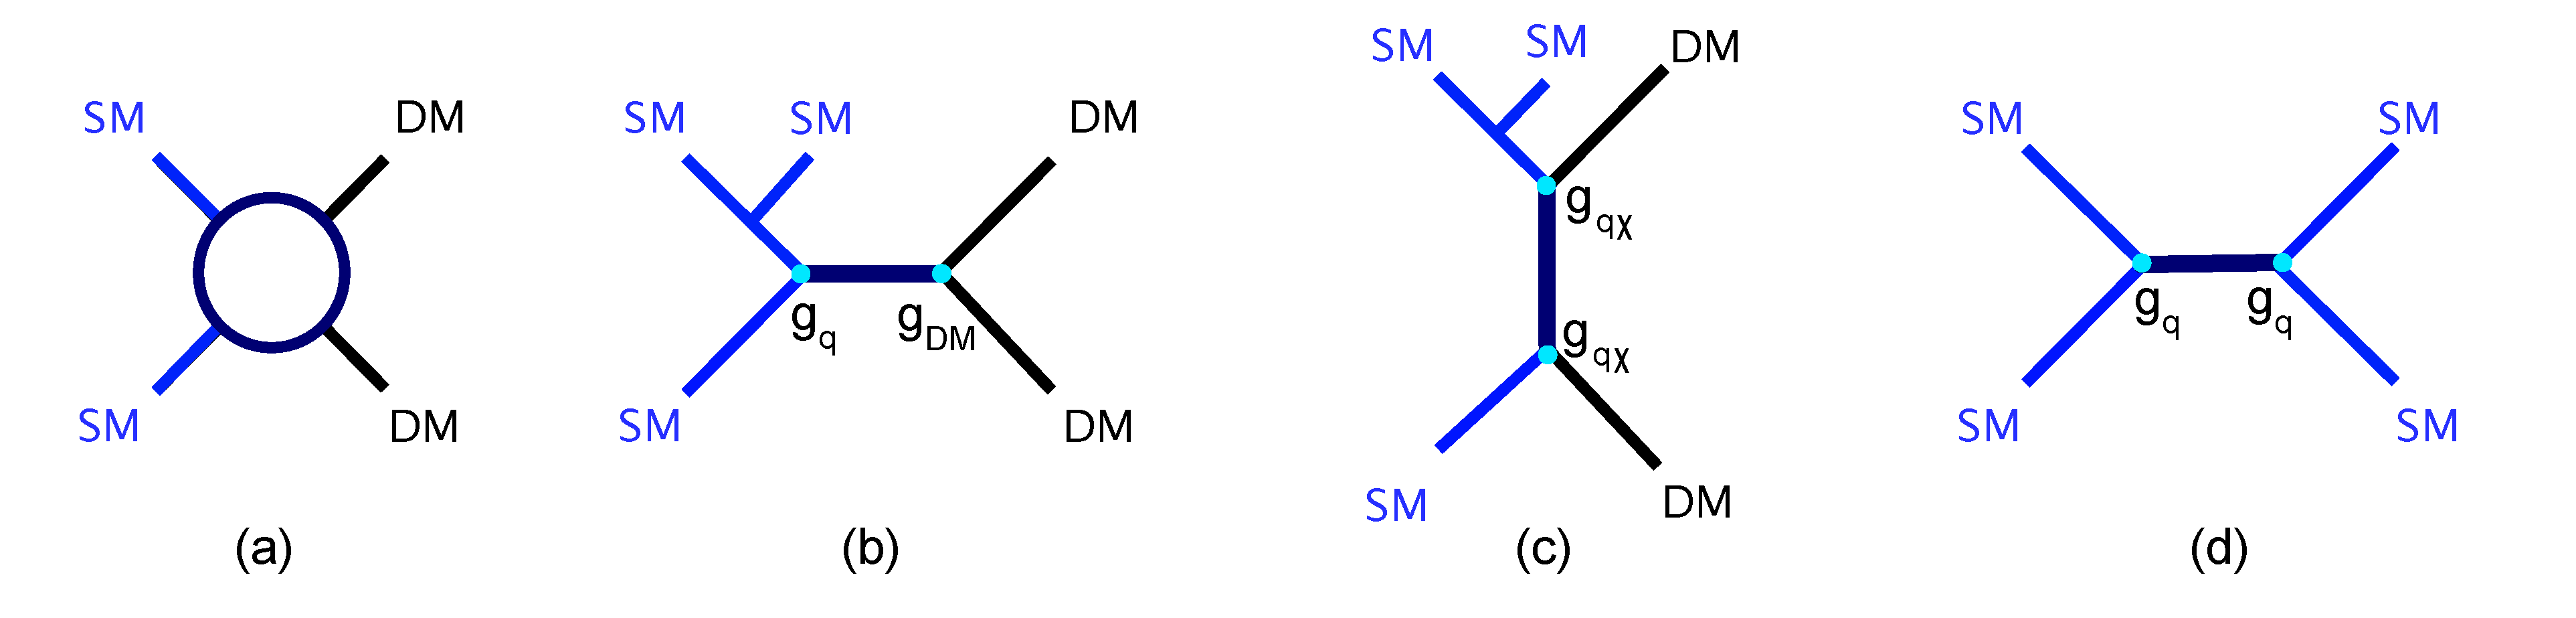
\includegraphics[width=\textwidth]{figures/feynman_0}

%\caption{

(\textit{a}) The interaction between DM\ and Standard Model particles via an unspecified interaction (e.g., an EFT).
(\textit{b}) Examples of simplified model processes where the interaction is mediated by an intermediate particle (with additional radiation off one of the initial-state quarks). 
(\textit{c}) The same model, in which  the mediator decays back into Standard Model particles, with coupling constant  \gq  for the mediator--quark--quark vertex and constant  \gdm for the mediator--DM vertex. 
Abbreviations:\ BSM, beyond the Standard Model; DM, dark matter; EFT, effective field theory; SM, Standard Model. \label{fig:feynman_0}

%}
%\end{figure}
